\appendix
\let\stdsection\section
\renewcommand\section{\newpage\stdsection}
\renewcommand{\thesection}{\Alph{section}}
\renewcommand*{\sectionmark}[1]{\markright{\MakeMarkcase{Anhang \thesection: #1}}}
\addcontentsline{toc}{chapter}{Anhang}

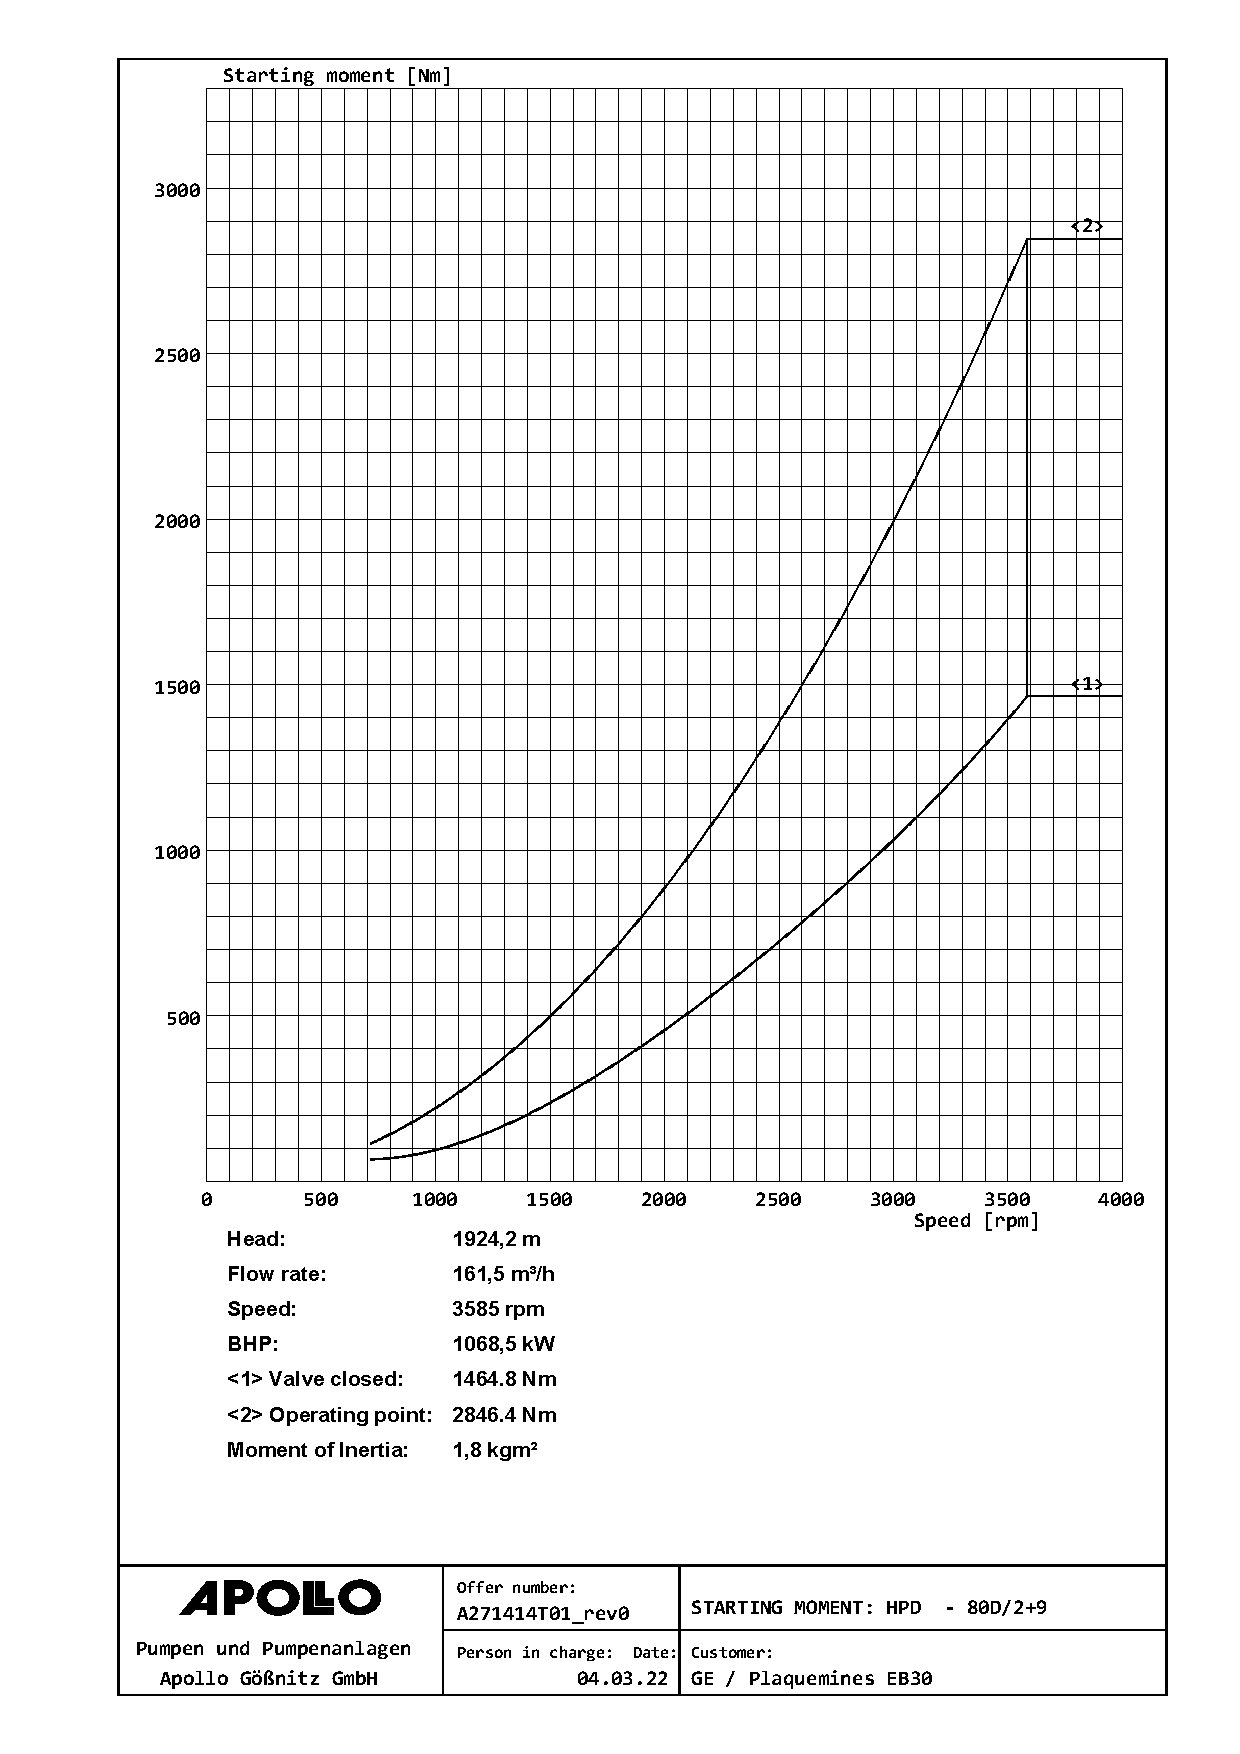
\includepdf[pages=-,scale = 0.8,
  pagecommand={},
  addtotoc={1,section,1,{Lastdrehmomentkurve},{app:lastdrehmoment}}
]{sections/appendix/lastdrehmoment.pdf}

\lstset{
    captionpos=top,
    language=C++,
    backgroundcolor=\color{white}
}

%Verbindung
\section{Quellcode MQTT und WiFi Verbindung}\label{sec:bib_mqtt_wlan}

\subsection{Header der Connection Library}
\lstinputlisting[label={lst:con_header},caption = ConnectionWiFi.h]{sections/appendix/ConnectionWifi/ConnectionWiFi.h}

